\documentclass[conference]{IEEEtran}
\IEEEoverridecommandlockouts
\setlength{\columnsep}{6mm}
\usepackage{hyperref}
\usepackage{cite}
\usepackage{amsmath,amssymb}
\usepackage{algorithmic}
\usepackage{graphicx}
\usepackage{textcomp}
\usepackage{xcolor}
\usepackage{stfloats}
\usepackage{booktabs}
\usepackage{url}
\usepackage{algorithm}
\usepackage{multirow}
\usepackage{flushend}
\usepackage{subfigure}
\usepackage{url}
\usepackage{pgfplots, tikz, amsmath, amssymb, tkz-euclide,tikz-layers,etoolbox,fontawesome5,colortbl}
\usetikzlibrary{intersections,calc, positioning,shapes}

\usepackage{array}
\newcolumntype{L}[1]{>{\raggedright\let\newline\\\arraybackslash\hspace{0pt}}m{#1}}
\newcolumntype{C}[1]{>{\centering\let\newline\\\arraybackslash\hspace{0pt}}m{#1}}
\newcolumntype{R}[1]{>{\raggedleft\let\newline\\\arraybackslash\hspace{0pt}}m{#1}}
% -------- for figures --------
\usepackage{tikz, pgfplots, graphicx, fontawesome5, colortbl, tabto, amssymb, amsmath, enumitem, lipsum, multirow, fancyhdr, array, xcolor, rotating}
\usetikzlibrary{shapes, calc, positioning, fit, decorations, decorations.text, arrows, arrows.meta}
\pgfplotsset{compat=1.17}  % i don't have 1.18 yet

% -------- end figures --------

%\usepackage{endnotes}
\usepackage{enotez}
\setenotez{list-name=References}
\let\footnote=\endnote
%\setlength{\parindent}{0pt}
\def\UrlBreaks{\do\A\do\B\do\C\do\D\do\E\do\F\do\G\do\H\do\I\do\J
	\do\K\do\L\do\M\do\N\do\O\do\P\do\Q\do\R\do\S\do\T\do\U\do\V
	\do\W\do\X\do\Y\do\Z\do\[\do\\\do\]\do\^\do\_\do\`\do\a\do\b
	\do\c\do\d\do\e\do\f\do\g\do\h\do\i\do\j\do\k\do\l\do\m\do\n
	\do\o\do\p\do\q\do\r\do\s\do\t\do\u\do\v\do\w\do\x\do\y\do\z
	\do\.\do\@\do\\\do\/\do\!\do\_\do\|\do\;\do\>\do\]\do\)\do\,
	\do\?\do\'\do+\do\=\do\#}
\makeatletter
\newcommand{\rmnum}[1]{\romannumeral #1}
\newcommand{\Rmnum}[1]{\expandafter\@slowromancap\romannumeral #1@}
\makeatother

\def\BibTeX{{\rm B\kern-.05em{\sc i\kern-.025em b}\kern-.08em
    T\kern-.1667em\lower.7ex\hbox{E}\kern-.125emX}}
\begin{document}

\title{{ZKLayer - A Verified Inference Network} \\

{\footnotesize}
}


\author{
\IEEEauthorblockA{{By: Colin Gagich, Ronald Chan, Spencer Graham, Will Prangley} \\
{Inference Labs Inc. - \url{inferencelabs.com}}\\
%E-mails: investor@inferencelabs.com
}
\IEEEauthorblockN{13 April 2024 (v1.1)}%, xyz i\IEEEauthorrefmark{1} and xyzi \IEEEauthorrefmark{1} and xyzz\IEEEauthorrefmark{1} and xyz\IEEEauthorrefmark{1}}

}
\maketitle

% change page style back to plain to enable page numbers
\thispagestyle{plain}
\pagestyle{plain}
% end of adding page numbers


\begin{abstract}
In contrast to Web2, characterized by its heavy reliance on centralized entities for data storage and processing, Web3 significantly reduces dependence on intermediaries, thereby mitigating risks associated with centralized data repositories. Through the integration of cryptographic principles and blockchain technology, Web3 prioritizes data sovereignty and enhances privacy. This decentralized framework fosters an environment where billions of individuals and machines can interact and collaborate without the oversight of central authorities, heralding a new era of democratic participation in society.

Meanwhile, Artificial Intelligence (AI) stands as a pivotal force shaping the future landscape of technology and society. Its importance lies not only in its ability to automate tasks and optimize processes but also in its capacity to revolutionize industries, drive innovation, and solve complex problems at scales previously unimaginable. From personalized medicine and autonomous vehicles to smart cities and predictive analytics, AI holds the potential to enhance efficiency, improve decision-making, and empower individuals and organizations to tackle global challenges.

In the Web3 environment, AI systems, like humans and other machines, should operate within a decentralized framework. The promising integration of AI capabilities within the decentralized framework of Web3 heralds the future, as this combination has the potential to unlock unprecedented levels of innovation, efficiency, and democratization. By leveraging this synergy, we can shape a more equitable and sustainable digital ecosystem for generations to come. However, while AI and Web3 each present their distinct challenges, their convergence brings about complex issues. Ensuring the responsible and ethical deployment of AI, preserving the integrity of inference, and safeguarding the intellectual properties of AI within the decentralized ecosystem of Web3 require addressing multifaceted concerns such as fairness and guarantees in payment, user privacy, and more.

This paper introduces ZKLayer, a decentralized network facilitating the deployment of AI systems on a Web3 infrastructure. In ZKLayer, we utilize cryptographic technologies such as zero-knowledge proofs (ZKP), fully homomorphic encryption (FHE), and multi-party computation (MPC) to safeguard the integrity and privacy of users and/or AI developers. Furthermore, a blockchain-based architecture ensures payment assurances and democratic governance within the system. While some challenges have been addressed, our team remains committed to continuously updating ZKLayer with new technologies to tackle emerging challenges in Decentralized AI.


\end{abstract}

%\begin{IEEEkeywords}  Blockchain; Data Sharing; SGX; Security; Privacy; Smart Contract

%\end{IEEEkeywords}

\section{Introduction}
\subsection{Background in AI and Web3}

This subsection provides a brief overview of AI and Web3.

\subsubsection{Artificial Intelligence (AI)} 


Artificial Intelligence (AI) stands at the forefront of modern technological advancements, revolutionizing industries and reshaping the way we interact with technology. With its ability to mimic human cognitive functions, AI enables machines to learn from data, adapt to new inputs, and perform tasks that traditionally required human intelligence. From personalized recommendation systems to autonomous vehicles, AI applications permeate various aspects of our daily lives, offering solutions to complex problems and unlocking new possibilities for innovation.


Machine Learning (ML), a subset of AI, focuses on the development of algorithms that allow computers to learn from and make predictions or decisions based on data. Through the iterative process of training on large datasets, ML algorithms can recognize patterns, extract insights, and improve their performance over time without being explicitly programmed. This capability is driving advancements in fields such as healthcare, finance, and cybersecurity, where ML techniques are being utilized to enhance diagnosic accuracy, optimize financial trading strategies, and detect anomalies in network traffic, among other applications. ML's versatility and effectiveness in handling large volumes of data make it a pivotal component of the AI landscape, propelling the evolution of intelligent systems and fueling the growth of data-driven decision-making across industries.

\subsubsection{Web3}

Web3 represents the next phase of the Internet through the emphasis on decentralization, transparency, and user empowerment. Unlike its predecessor, Web2, which is characterized by centralized platforms and gatekeepers, Web3 aims to distribute power and control back to individual users through blockchain technology and decentralized protocols. In the Web3 ecosystem, users have greater ownership and control over their data and digital assets, facilitated by cryptographic principles and smart contracts. This shift towards decentralization not only reduces reliance on intermediaries but also fosters trust and security by design, as transactions are recorded on a transparent and immutable ledger. As a result, Web3 enables new models of digital interaction, including decentralized finance (DeFi), non-fungible tokens (NFTs), and decentralized autonomous organizations (DAOs), which offer innovative ways for individuals to engage, transact, and collaborate online.

Moreover, Web3 holds the potential to democratize access to information and resources, empowering individuals across the globe to participate in the digital economy on their own terms. By leveraging decentralized networks and peer-to-peer interactions, Web3 can circumvent censorship, promote financial inclusion, and facilitate cross-border transactions without the need for traditional intermediaries. Additionally, Web3 technologies such as decentralized storage and identity solutions provide avenues for individuals to regain control over their digital identity and secure their online presence. As the Web3 ecosystem continues to evolve and mature, it has the capacity to redefine the Internet as a more open, inclusive, and equitable space, where individuals have greater agency and autonomy in shaping their digital experiences and interactions.


\subsection{The rationale for the combination of AI and Web3}
The combination of AI and Web3 technologies holds immense potential to revolutionize various aspects of our digital landscape. By integrating AI with decentralized protocols and blockchain systems, we can leverage the strengths of both domains to create more efficient, secure, and transparent systems. One significant benefit lies in the realm of DeFi, where AI algorithms can analyze vast amounts of data from blockchain networks to optimize trading strategies, detect fraudulent activities, and provide personalized financial services. Additionally, AI-powered smart contracts can automate complex processes, such as loan approvals or asset management, without the need for intermediaries, enhancing the speed and accuracy of transactions while reducing costs and human errors.

Furthermore, the combination of AI and Web3 technologies can foster greater privacy and data ownership for users. AI algorithms can be deployed within decentralized applications (dApps) to provide personalized experiences while preserving user anonymity and data sovereignty. For instance, AI-driven recommendation systems can suggest content or products based on user preferences without compromising privacy by processing data directly on the user's device or utilizing privacy-enhancing techniques. Moreover, integrating AI with decentralized identity solutions can enhance identity verification processes while ensuring user control over their personal data. This symbiotic relationship between AI and Web3 not only enhances the efficiency and security of digital interactions but also empowers individuals to reclaim ownership of their digital identities and data in an increasingly decentralized and interconnected world.

\subsection{Overviewing all challenges}

Combining AI with Web3 technologies presents a complex and multifaceted challenge. Integrating AI algorithms into decentralized systems requires careful consideration of compatibility, interoperability, and scalability. AI models often rely on vast amounts of data for training and inference, posing significant challenges in terms of data privacy, storage, and access within decentralized networks. Moreover, ensuring the transparency and fairness of AI-driven processes in a decentralized environment is inherently difficult, as traditional centralized oversight mechanisms may not be applicable. Additionally, the dynamic and rapidly evolving nature of both AI and blockchain technologies introduces complexities in maintaining compatibility and synchronization between the two domains. Addressing these challenges requires interdisciplinary expertise spanning AI, cryptography, blockchain, and distributed systems, making the integration of AI and Web3 a formidable endeavor that demands innovative solutions and collaborative efforts from experts across various fields.

On the one hand, AI offers transformative capabilities in enhancing efficiency, decision-making, and user experiences. However, it also brings forth significant challenges related to privacy, integrity, security, and so on. The inherent opacity of AI models, coupled with concerns regarding data privacy and algorithmic bias, raises questions about the ethical implications and trustworthiness of AI-driven systems. Moreover, ensuring the integrity and security of AI algorithms and datasets is paramount to mitigate the risks of adversarial attacks, data manipulation, and unauthorized access.

Similarly, Web3 introduces its own set of challenges, particularly concerning privacy and data protection. Decentralized networks aim to empower users with greater control over their data and digital identities. However, achieving privacy in a transparent and auditable blockchain environment presents inherent tensions. While cryptographic techniques such as zero-knowledge proofs offer promising solutions, they also introduce complexities in terms of implementation, scalability, and usability. Additionally, navigating regulatory frameworks and compliance requirements in decentralized ecosystems poses challenges in ensuring legal and regulatory compliance while preserving user privacy and data sovereignty.

Despite the individual challenges posed by AI and Web3, the combination of the two further compounds the complexity. Integrating AI algorithms into decentralized networks requires addressing the unique challenges of both domains while ensuring compatibility, security, and usability. The interoperability between AI and Web3 technologies necessitates novel approaches to data privacy, algorithmic transparency, and governance mechanisms. As such, achieving a seamless and effective fusion of AI and Web3 requires a concerted efforts to overcome technical, regulatory, and societal challenges, making it a highly intricate and demanding undertaking.

\subsection{Ensuring Practicality: A Comprehensive Solution}

To effectively address the multifaceted challenges arising from the integration of AI and Web3 technologies, a practical solution must encompass a diverse range of essential capabilities. These include:


\begin{enumerate}

    \item \textbf{Authentication:} Implementing robust authentication mechanisms to verify user identities and maintain the integrity of interactions within decentralized networks.

    \item \textbf{Privacy Preservation:} Ensuring the protection of sensitive data and preserving user privacy through encryption, anonymization techniques, and privacy-enhancing technologies.

    \item \textbf{Security Measures:} Incorporating comprehensive security protocols to safeguard against data breaches, cyber-attacks, and unauthorized access, bolstering the overall resilience of the system.

    \item \textbf{Scalability Solutions:} Developing scalable architectures and protocols to accommodate the growing volume of data and transactions processed by AI-powered applications on Web3 platforms.

    \item \textbf{Fairness Assurance:} Implementing measures to ensure the fairness and transparency of AI algorithms and decision-making processes, mitigating biases and promoting inclusivity.

    \item \textbf{Decentralization:} Upholding the principles of decentralization to enhance transparency, resilience, and user autonomy, reducing reliance on central authorities and intermediaries.

    \item \textbf{Interoperability:} Facilitating seamless interoperability between different AI models, blockchain networks, and decentralized applications to enable efficient data exchange and collaboration.

    \item \textbf{Governance Mechanisms:} Establishing transparent governance frameworks to govern the operation and evolution of the system, enabling community-driven decision-making and consensus-building.

    \item \textbf{Data Sovereignty:} Empowering users with greater control over their data and digital identities, enabling them to manage and monetize their personal information in a secure and transparent manner.

    \item \textbf{Regulatory Compliance:} Ensuring compliance with relevant regulations and legal frameworks governing data protection, privacy, and financial transactions, fostering trust and legitimacy in the system.

    \item \textbf{Auditability:} Establishing mechanisms for auditing and verifying the integrity of transactions, data, and AI algorithms, enabling thorough examination and verification processes to ensure accuracy and compliance.

    \item \textbf{Transparency:} Promoting openness and visibility in the operation and decision-making processes of the system, enhancing accountability and trustworthiness by making relevant information accessible to stakeholders.

    \item \textbf{Robustness:} Building resilient architectures and protocols capable of withstanding various threats and disruptions, ensuring the continuous operation of the system under adverse conditions.

    \item \textbf{Updatability:} Ensuring the system's capacity to integrate and adapt to emerging technologies, fostering continuous innovation and resilience against obsolescence.

\end{enumerate}

By incorporating these diverse capabilities into a holistic framework, a practical solution can effectively address the complex challenges posed by the convergence of AI and Web3, laying the groundwork for the development of innovative and trustworthy decentralized applications.

\subsection{Our contribution}

Designing a system that effectively addresses all of the mentioned challenges and provides all of the capabilities outlined is undoubtedly a formidable task. However, we recognize the complexity of this endeavor and acknowledge that achieving the ideal solution may not be feasible from the outset. Instead, our approach entails starting with a system that addresses some of the pressing issues and then iteratively updating and enhancing it with new technologies and functionalities over time. By adopting this iterative approach, we aim to incrementally improve the system's capabilities and resilience, ultimately working towards the overarching goal of providing a comprehensive solution that fulfills all requirements and effectively integrates AI and Web3 technologies. This adaptive strategy allows us to navigate the complexities of technological evolution while ensuring that the system remains agile and responsive to emerging challenges and opportunities.

Our proposed system, ZKLayer, aims to leverage blockchain technology to facilitate the exchange of inferences between model developers and users in a secure and transparent manner. Through the ZKLayer network, model developers can offer their trained models to users seeking specific predictions or analyses. Users, in turn, can access these inferences by paying with tokens which then creates a decentralized marketplace for AI services. To ensure the integrity and trustworthiness of the exchanged inferences, model developers utilize zero-knowledge proofs (ZKPs) to provide verifiable evidence that the requested computations were indeed performed correctly without revealing any sensitive information about the underlying model or data. By integrating ZKPs into the transaction process, our system enhances transparency and trust, enabling users to confidently engage with model developers while preserving the confidentiality of their data and ensuring the authenticity of the provided inferences. Through this innovative blockchain-based solution, we aim to empower both model developers and users to participate in a secure and efficient marketplace for AI services, fostering a decentralized ecosystem that promotes fairness, transparency, and collaboration.

\section{Technological Foundations: Exploring Key Technologies}
To integrate AI and Web3 and provide a comprehensive list of capabilities, we explore various technologies in this section. Some of these technologies are utilized in designing ZKLayer version 1, while others are not yet practical for implementation. However, it's essential to note that ZKLayer will continually update to incorporate any advancements in technologies to evolve into a more practical solution over time.

\subsection{Technologies used in ZKLayer 1.0}

This subsection delves deeper into describing the technologies utilized in designing ZKLayer 1.0.

\subsubsection{Blockchain}

Blockchain technology, initially introduced as the underlying technology for cryptocurrencies like Bitcoin~\cite{Nakamoto2008BitcoinPeerToPeer}, has evolved into a revolutionary tool with diverse applications across various industries. At its core, blockchain is a decentralized, immutable ledger that records transactions in a transparent and secure manner. Its distributed nature eliminates the need for intermediaries, reducing transaction costs and increasing efficiency. One of the key benefits of blockchain is its transparency, as all transactions are recorded on a public ledger accessible to all participants, fostering trust and accountability.

Additionally, blockchain offers enhanced security through cryptographic techniques, making it highly resistant to tampering and fraud. Furthermore, blockchain facilitates peer-to-peer transactions without the need for centralized authorities, empowering individuals to directly exchange value and assets. Overall, blockchain technology has the potential to streamline processes, increase transparency, and democratize access to services, thereby revolutionizing numerous sectors and driving innovation.

\subsubsection{Smart Contract}

Smart contracts, a pivotal innovation enabled by blockchain technology, are self-executing contracts with the terms of the agreement directly written into code. Operating on decentralized networks like Ethereum, smart contracts automate and enforce the execution of contractual agreements without the need for intermediaries, thereby reducing reliance on traditional legal processes and enhancing efficiency. These programmable contracts can execute predefined actions automatically when specific conditions are met, facilitating a wide range the tokenization of assets, DeFi, supply chain management, and more. By leveraging cryptographic security and decentralization, smart contracts ensure trust and immutability, as transactions are recorded on a tamper-proof blockchain ledger. This transformative technology has the potential to revolutionize the way agreements are made and executed, offering increased transparency, speed, and reliability in various industries and sectors.

\subsubsection{Blockchain interconnection}

Blockchain interconnection, as a critical component for designing ZKLayer, refers to the capability of various blockchain networks or platforms to communicate and interact seamlessly. This interoperability facilitates the smooth flow of data, assets, or transactions between disparate blockchain systems, fostering cross-chain functionality and collaboration. There are multiple approaches to achieving blockchain interconnection, including cross-chain communication protocols, atomic swaps, wrapped tokens, sidechains, and oracles. Such interconnection is pivotal for unlocking the complete potential of blockchain technology, enabling collaboration, scalability, and interoperability across diverse blockchain networks and platforms.

\subsubsection{ZKP}

Zero-knowledge proof (ZKP) represents a breakthrough cryptographic technique that enables one party to prove the validity of a statement to another party without revealing any additional information beyond the validity itself. This powerful concept allows for the verification of data or computations while maintaining the privacy and confidentiality of sensitive information.

\subsubsection{ZKML}

In the realm of cutting-edge cryptographic technologies, Zero-Knowledge Machine Learning (ZKML) emerges as a game-changer by combining the power of zero-knowledge proofs with machine learning algorithms. Not all challenges in AI and ML but some of them could be addressed through ZKP.

One significant challenge within the Machine Learning as a Service (MLaaS) industry pertains to the integrity of inferences, where clients seek assurance that the model developer has genuinely executed the requested model for their response. For example, consider a client purchasing a premium account from OpenAI to utilize ChatGPT 4. They may question whether OpenAI could opt to use the cheaper ChatGPT 3 instead, thereby saving costs but potentially compromising the quality of responses to a level that the customer cannot distinguish. Similarly, when a patient consults an AI doctor for health predictions, concerns arise about the authenticity of the executed model. Even if the AI doctor acts with honesty, the risk of system compromise, where a genuine model may be replaced with a poisoned one by hackers, poses a serious threat. In both instances, maintaining the integrity of the model remains a paramount concern for the customer.

A naïve solution would involve the model developer sharing the model with the customers, who would then run the model locally to ensure its integrity. However, this approach is not practical due to the large size of models and the limited computational resources available to customers. As an alternative, Ghodsi et al.~\cite{Ghodsi2017SafetyNetsVE} proposed, for the first time, the use of ZKP to design a solution where the model developer, or a third party like a cloud service, runs the model but generates a proof using ZKP for the customer to ensure that the genuine model has been executed.

While Ghodsi's solution offers benefits, it necessitates the sharing of the model with customers. However, in certain scenarios, model developers may be reluctant to share their models due to concerns about protecting intellectual property. Consequently, in addition to ensuring the integrity of the model, preserving the privacy of the model becomes another significant concern. Thus, the overarching question arises: How can model developers assure customers that the model has been genuinely executed (ensuring the integrity of inference) without divulging any information about the model itself (preserving model privacy)? To address this new complicated problem, Lee et al.~\cite{Lee2020vCNNVC} proposed a ZKP-based solution that aims to addresse both concerns. Subsequently, other researchers have proposed a more efficient ZKP-based solution to address these two concerns~\cite{Liu2021zkCNNZK},~\cite{Feng2021ZENAO},~\cite{Ju2021EfficientSP}.

% FIXME: bad wording "provide both concern"



\section{ZKLayer}

Zero-Knowledge Layer (ZKLayer) offers a transformative approach for AI operators seeking to transition their off-chain AI models onto blockchain networks while safeguarding their proprietary algorithms. This framework streamlines the intricate process of model conversion, enabling rapid deployment across multiple blockchain ecosystems. It serves as a seamless bridge between the off-chain world of AI and the on-chain realm, ensuring intellectual property remains veiled through the use of zero-knowledge cryptography. By providing a secure and efficient payment infrastructure, ZKLayer facilitates atomic value exchange for AI services, paving the way for a new era of autonomous AI agents interacting within the blockchain space.

For consumers of AI predictions, ZKLayer offers an additional layer of assurance by eliminating trust assumptions. They confidently rely on the network to validate that the inputs are processed using the correct and intended AI model, with a cryptographic guarantee of faithful execution.  As a result, consumers of AI services benefit from a transparent, trust-minimized environment where AI predictions are verified, reducing the need for blind trust in the operators' execution.

\subsection{Technical Architecture}

To address current blockchain limitations and challenges of running on-chain Neural Networks, ZKLayer is designed to serve as a conduit between off-chain and on-chain architectures. Taking a forward-looking approach, the ZKLayer architecture is inherently modular, a design philosophy that allows each component of the system to be individually updated or replaced.

\begin{figure}[!ht]
    \centering
    \scalebox{0.50}{
\tikz{
\tikzstyle{block}=[draw, inner sep=0pt, outer sep=0pt, minimum width=4cm, minimum height=2.3cm, rounded corners=2mm, align=center, font=\small]

\node[block] (mr)  {Model Registry\\[2mm]Model A\\Model B\\Model C};
\node[block, right=1.7cm of mr] (np)  {Inference Market\\(workload queue)};
\node[block, right=1.7cm of np] (ua)  {ZKLayer SDK\\$1:1$ verifier contract per\\model\\Verifying Keys\\Verified Output Data};

\node[block, below=3cm of mr] (mr1)  {Node Pool\\(workers)};
\node[block, right=1.7cm of mr1] (np1) {zk-ML proving circuits\\(model dependant)};
\node[block, right=1.7cm of np1] (ua1)  {Aggregation Circuits\\(proof of proofs)};

\node[block, minimum height=1.2cm, above=.7cm of np, rounded corners=6mm] (eu) {End Users\\
Al prediction consumers};
\node[block, minimum height=1.2cm, above=.7cm of ua, rounded corners=6mm] (da) {dApp Contract};

\node[cylinder, draw, shape aspect=1, minimum height=1cm,
       minimum width=1.8cm, minimum height=1.5cm, rotate=90] (cy) at ([yshift=-2.5cm]$(mr1)!.5!(np1)$) {} node at (cy) {Arweave};

\node[draw, anchor=north, minimum width=17cm, minimum height=5.5cm, rounded corners=3mm] (r1) at ([yshift=1cm]np1.north) {};
\node[draw, dashed, anchor=south, minimum width=17cm, minimum height=5.4cm, rounded corners=3mm] (r2) at ([yshift=-1cm]np.south) {};

\node[above right, anchor=south west] at (r1.north west) {\textbf{off-chain}};
\node[above right, anchor=south west] at (r2.north west) {\textbf{on-chain}};
% Paths
\draw[-triangle 45] (eu)--(np); \draw[-triangle 45] (da)--(ua);
\draw[-triangle 45] (da.west) -- ++(-1,-.85) -| (np.60);
\draw[-triangle 45] (ua)-- node[align=center,below, font=\footnotesize] {Prune\\Completed\\Workloads} (np);
\draw[-triangle 45] (mr)--node[fill=white,pos=.17] {Model Details} (mr1);
\draw[-triangle 45] (np.-100)--node[fill=white, pos=.33] {Input} ++(0,-1.5) -|  (mr1.60);
\draw[-triangle 45] (np1.80)--node[fill=white, pos=.33] {Proof \& Output} ++(0,1.5) -|  (ua.-120);
\draw[-triangle 45] (ua1)--node[fill=white, pos=.17] {Proof(s) \& Output(s)}   (ua);
\draw[-triangle 45] (mr1)--node[above] {Output} coordinate[pos=.5] (z) (np1);
\draw[-triangle 45] (np1)--node[above] {Proofs} (ua1);
\draw[-triangle 45] (z)--(cy);
}
}
    \caption{ZKLayer Overview}
    \label{fig:Fig 1}
\end{figure}

This adaptability is a core characteristic, anticipating the need to integrate advanced AI models and alternative solutions as they emerge in the dynamic AI and blockchain landscape.

\subsection{Off-Chain Architecture}

\textit{Node Pools: }The off-chain infrastructure and computational power of ZKLayer is based around node pools.

\begin{figure}[!ht]
    \centering
    \scalebox{0.50}{
\tikz{
\tikzstyle{block}=[draw, inner sep=0pt, outer sep=0pt, minimum width=1.8cm, minimum height=1.2cm, rounded corners=1mm, align=center, fill=black!50]

\node[draw, densely dotted, thick, minimum width=8cm, minimum height=1.7cm, rounded corners=2mm] (r1) at (0,0)  {};
\node[draw, densely dotted, thick, minimum width=8cm, minimum height=1.7cm, rounded corners=2mm, left=3mm of r1] (r2) {};

\node[fill=white, anchor=west, xshift=2mm] at (r2.north west) {\footnotesize\textbf{Node Pool}};

\node[block, anchor=west, text=white] (a) at ([xshift=3mm]r1.west) {Node A};
\node[block,right=.3cm of a, text=white] (b) {Node B};

\node[block, anchor=west, text=white] (a1) at ([xshift=3mm]r2.west) {Node A};
\node[block,below=.55cm of a1, text=white] (b1) {Node B};
% %---------
\node[minimum width=1.75cm, minimum height=1.2cm, anchor=south west] (1) at ([yshift=3mm]r2.north west) {};
\draw (1.north west)--coordinate[pos=1] (w) ($(1.west)+(.5,0)$)--(1.south west)--(1.south east)--coordinate[pos=1] (z) ($(1.east)+(.5,0)$)--(1.north east)--cycle;
\node[align=center, font=\scriptsize] at($(w)!.4!(z)$) {Workload\\1};

\node[minimum width=1.75cm, minimum height=1.2cm, right=1.3mm of 1] (1) {};
\draw (1.north west)--coordinate[pos=1] (w) ($(1.west)+(.5,0)$)--(1.south west)--(1.south east)--coordinate[pos=1] (z) ($(1.east)+(.5,0)$)--(1.north east)--cycle;

\node[minimum width=1.75cm, minimum height=1.2cm, right=1.3mm of 1] (1) {};
\draw (1.north west)--coordinate[pos=1] (w) ($(1.west)+(.5,0)$)--(1.south west)--(1.south east)--coordinate[pos=1] (z) ($(1.east)+(.5,0)$)--(1.north east)--cycle;
\node[align=center, font=\scriptsize] at($(w)!.4!(z)$) {Workload\\2};

\node[minimum width=1.75cm, minimum height=1.2cm, right=1.3mm of 1] (1) {};
\draw (1.north west)--coordinate[pos=1] (w) ($(1.west)+(.5,0)$)--(1.south west)--(1.south east)--coordinate[pos=1] (z) ($(1.east)+(.5,0)$)--(1.north east)--cycle;
\node[align=center, font=\scriptsize] at($(w)!.4!(z)$) {Workload\\3\\Workload\\4};



\node[minimum width=1.75cm, minimum height=1.2cm, anchor=south west] (1) at ([yshift=3mm]r1.north west) {};
\draw (1.north west)--coordinate[pos=1] (w) ($(1.west)+(.5,0)$)--(1.south west)--(1.south east)--coordinate[pos=1] (z) ($(1.east)+(.5,0)$)--(1.north east)--cycle;
\node[align=center, font=\scriptsize] at($(w)!.4!(z)$) {Workload\\5};

\node[minimum width=1.75cm, minimum height=1.2cm, right=1.3mm of 1] (1) {};
\draw (1.north west)--coordinate[pos=1] (w) ($(1.west)+(.5,0)$)--(1.south west)--(1.south east)--coordinate[pos=1] (z) ($(1.east)+(.5,0)$)--(1.north east)--cycle;
\node[align=center, font=\scriptsize] at($(w)!.4!(z)$) {Workload\\6};

\node[minimum width=1.75cm, minimum height=1.2cm, right=1.3mm of 1] (1) {};
\draw (1.north west)--coordinate[pos=1] (w) ($(1.west)+(.5,0)$)--(1.south west)--(1.south east)--coordinate[pos=1] (z) ($(1.east)+(.5,0)$)--(1.north east)--cycle;
\node[align=center, font=\scriptsize] at($(w)!.4!(z)$) {Workload\\7\\Workload\\8};

\node[minimum width=1.75cm, minimum height=1.2cm, right=1.3mm of 1] (1) {};
\draw (1.north west)--coordinate[pos=1] (w) ($(1.west)+(.5,0)$)--(1.south west)--(1.south east)--coordinate[pos=1] (z) ($(1.east)+(.5,0)$)--(1.north east)--cycle;
\node[align=center, font=\scriptsize] at($(w)!.4!(z)$) {Workload\\9\\Workload\\10};

%---------------
\node[above=1.6cm] at (r2.north) {Epoch 1};
\node[above=1.6cm] at (r1.north) {Epoch 2};
% Paths
\draw[-triangle 45] (b1)-| node[pos=.25, fill=white] {\small \textbf{Node Registers based on workload}} (b);
}
}    \caption{Epoch transition with new Node registration}
    \label{fig:Fig 2}
\end{figure}

These pools consist of registered nodes that are assigned to process specific models' inference workloads. After registration, a model node becomes part of the available workforce. A node may service multiple models, and it is incumbent upon the node operator to ensure the successful completion of assigned tasks. Nodes pledge a certain amount of computational power and time to the network. With the computational requirements of workloads being predetermined, the network allocates tasks accordingly and does not exceed a node's capacity. A node is expected to fulfill its commitments within the epoch it is registered. Any failure to perform, or indication of unavailability, may result in penalties to the node.


\subsection{Persistent Storage}

Due to the considerable size of input and outputs from AI models, external persistent storage is required. Depending on the ultimate end use case of the output, storage within ZKLayer may not be required. An example is an NFT image generated with a diffusion model. The hash of the image can be verified and stored on-chain with the image being stored on Arweave~\cite{Arweave} or other decentralized storage networks.


\subsection{Aggregation Circuits}

As the complexity of a model increases, so does the size of its associated zk-circuit which results in larger proofs. To manage this, aggregation circuits are utilized to amalgamate multiple proofs into a singular, more concise proof that can be submitted on-chain, along with the corresponding output data. This technique also permits the batching of related inferences, enhancing efficiency and reducing the on-chain data storage footprint.

\subsection{On-chain Architecture}

The on-chain component of the ZKLayer system acts as the interface for end users and dApps.  Users or dApps submit workloads, which include all necessary details like input, precommitment, and destination. This on-chain architecture consists of three main components: The Inference Market, Model Registry, and Verifier Contracts.

\subsection{Inference Market}

The ecosystem is anchored by an Inference Market. The protocol has a native queue of AI/ML workloads. A workload can be thought of as an end-to-end AI/ML Inference. Each workload specifies all required details to complete it, such as input data, specific AI model for execution, output data requirements or on-chain execution. Workloads posted to the network are priced according to their computational complexity.

\subsection{Model Registry}

After circuitizing a model with the ZKLayer SDK, its creator will register it on the network. This defines the required input and output data format, computational cost of inferences on the model (proportional to cost of compute for an inference) and the verification key for use in a verification contract upon completion of each inference from the model.

\subsection{Model Node Pool Registration}

In order to complete inference workloads for a model, a model node must register its intent to complete workloads for specific models. Once registered the node is added to the pool of available nodes. Nodes may be registered to service multiple models, but it is the responsibility of the operator to ensure the node completes assigned workloads.

\begin{figure}[!ht]
    \centering
\scalebox{0.65}{
\tikz{
\tikzstyle{block}=[draw, inner sep=0pt, outer sep=0pt, minimum width=2.2cm, minimum height=1.2cm, rounded corners=1mm, align=center]

\node[block, fill=black!50, text=white] (a) {Model A};
\node[block, fill=black!50, text=white, right=.5cm of a] (b) {Model B};
\node[block, fill=black!50, text=white, below=.5cm of a] (c) {Model C};

\node[block,  left=2cm of a] (na) {Node A};
\node[block,  below=.5cm of na] (nb) {Node B};

%---------
\coordinate (p) at ($(a.west)!.5!(c.west)$);
\node[draw, dashed, anchor=west, minimum width=5.8cm, minimum height=3.5cm, rounded corners=2mm, label={above:Node Pool}] at ($(p)+(-.5,0)$)  {};
%-------------
\draw[-triangle 45] (na)--(a);
\draw[-triangle 45] (nb)--(c);
\draw[-triangle 45] (nb.east)--++(.7,0) |- (a.195);
}
}
    \caption{Model Registration}
    \label{fig:Fig 3}
\end{figure}

The network implements sets of blocks, called epochs, in which a registered node must be available. Nodes that register in the current epoch are activated during the following epoch. Model nodes commit compute units per unit of time to the network. Since the compute units for a workload are known ahead of time the network delegates workloads to fill but not exceed its compute capacity.

It is the expectation that a model node will complete delegated workloads during a registered epoch. Model nodes that fail to complete work while registered or otherwise shown to be unavailable will face a penalty.

\subsection{Model Vetting}

As ZKLayer will be an open permission-less network, no party (or even Inference Labs) can decide which models should or shouldn’t be available on the network. Instead an economic system determines how “good” a model is. This is crucial to retain an open and fair censorship free network.

Verified backtesting is published by the model creator and made available to the public. Users get a guarantee the model will perform a certain way under set circumstances rather than relying on blind trust in published accuracy, precision and recall values. While the provided examples may not be representative of real-world use cases as it is self-published by the creator, this can be seen as a move in the right direction. Users also submit inferences one at a time, with no upfront commitments or complicated setup to quickly verify the usefulness of the model for their application.

Aggregating on-chain historical usage of a model results in a proof of its usefulness. How “good” a model is can be answered by its frequency of use, inference by a diverse set of applications and users, and repeat use of a model by a user. In the same way an open-source software package can be evaluated by the number of other projects that depend on it (and subsequently how “good” those packages are).

The network implements a non-zero registration fee for models to prevent flooding of the network with unusable or non-existent models.


\section{Current Execution and Deployment}

This section provides an overview of the implementations undertaken by the team. Our team has assessed some projects (consisting EZKL, RISC0, ORION and KANG) focused on providing AI solutions to compare and evaluate their performance, as outlined in~\cite{BrainbenchXYZ} along with detailed information. The following table compares various ZKML projects based on different properties.

\begin{figure}[!ht]
    \begin{tikzpicture}[font=\normalsize]
\def\vlt{blue!50!violet}
\def\tg{teal!70!green}
\def\check{\color{\tg}\small\faCheck}
\def\cross{\color{red!80!black}\small\faTimes}
\def\info{\color{gray!40}\small\faInfoCircle}
\def\circle{\color{orange!30!yellow}\small\faCircle}
\def\excla{\color{yellow!50!olive}\footnotesize\raisebox{0.3mm}{\faExclamationTriangle}}

\node[] {
\renewcommand{\arraystretch}{1.6}
\arrayrulecolor{gray}
\hspace{-4.5mm}
\footnotesize
\begin{tabular}{|>{\raggedright\arraybackslash}>{\centering\arraybackslash}p{2cm}>{\centering\arraybackslash}p{0.87cm}>{\centering\arraybackslash}p{0.87cm}>{\centering\arraybackslash}p{0.87cm}>{\centering\arraybackslash}p{2cm}|}
\hline
\textbf{PROPERTY} & \textbf{EZKL}  & \textbf{RISC0} & \textbf{ORION} & \textbf{DANIEL KANG'S ZKML}  \\
\hline
\textbf{Source language}  & Rust & Rust & Cairo & Rust  \\
\hline
\textbf{Version}  & 8.1.7 & v0.19.1 & v0.2.2 & main@4378958  \\
\hline
\textbf{API Support}  &  &  &  &   \\
\hline
\textbf{Python}  & \check & \cross & \cross & \cross\quad\excla  \\
\hline
\textbf{Javascript}  & \check & \cross & \cross & \cross\quad\excla  \\
\hline
\textbf{Rust}  & \check & \check & \check &  \cross\quad\excla \\
\hline
 \textbf{Others}  & WASM & \circle & \cross & \cross  \\
\hline
\textbf{ZK Proving System}  & SNARK & STARK & STARK & SNARK  \\
\hline
\textbf{Unbounded Models}  & \cross & \check & \cross & \cross  \\
\hline
\textbf{Randomness Operations}  & \cross & \check & \cross & \cross \\
\hline
\textbf{Audit}  & \cross & \cross & \cross &  \cross \\
\hline
\textbf{Native Model Format}  & ONNX & Rust, C$++$ & ONNX & msgpack   \\
\hline
\textbf{Supported Operators}  & 89\%  & 100\% & 51\%  & 20\%   \\
\hline
\textbf{GPU Acceleration}  &  &  &  &   \\
\hline
\textbf{CUDA}  & \check\quad & \check\quad\excla & \cross & \cross  \\
\hline
 \textbf{Metal}  & \cross & \check & \cross &  \cross \\
\hline
\end{tabular}
};
\end{tikzpicture}
    \label{fig:Fig a}
\end{figure}

In addition to assessing various properties, our team has evaluated the performance of the underlying ZKP systems within the projects, as depicted in the following figure.

\begin{figure}[!ht]
    \centering
   \begin{tikzpicture}[font=\normalsize]
\def\vlt{blue!50!violet}
\def\tg{teal!70!green}
\def\check{\color{\tg}\small\faCheck}
\def\cross{\color{red!80!black}\small\faTimes}
\def\info{\color{gray!40}\small\faInfoCircle}
\def\circle{\color{orange!30!yellow}\small\faCircle}
\def\excla{\color{yellow!50!olive}\footnotesize\raisebox{0.3mm}{\faExclamationTriangle}}


\node[] {
\renewcommand{\arraystretch}{1.6}
\arrayrulecolor{gray}
\hspace{-5mm}
\footnotesize
\begin{tabular}{|>{\raggedright\arraybackslash}p{1.9cm}>{\centering\arraybackslash}p{2.1cm}>{\centering\arraybackslash}p{1.3cm}>{\centering\arraybackslash}p{1.7cm}|}
\hline
\textbf{8 Cores, 32 GB RAM, CUDA Accelerator} & \textbf{10 Cores, 32 GB RAM, Metal Accelerator} & \textbf{EZKL's Lilith} & \textbf{64 Cores, 128 GB RAM}  \\
\hline
BENCHMARK & \multicolumn{1}{c}{EZKL}  & \multicolumn{1}{c}{RISC0} & \multicolumn{1}{c|}{ORION}  \\
\hline
\textbf{Linear regressions}  &  &  &   \\
\hline
 \textbf{Proof Size}  & 4.88kB & 58.18 kB & No data  \\
\hline
\textbf{Proof Memory Usage}  & 9.93 MB & 1.25 GB & 55.21 MB  \\
\hline
 \textbf{Proof Time}  & 251.00ms & 43 seconds & 707.50ms  \\
\hline
\textbf{Random forests}  &  &  &   \\
\hline
\textbf{Proof Size}  & 9.13 kB & 67.27 kB & No data   \\
\hline
 \textbf{Proof Memory Usage}  & 440.43 MB & 9.75 GB & No data  \\
\hline
\textbf{Proof Time}  & 4 seconds & No data &  No data \\
\hline
\textbf{Svm classifications}  &  &  &   \\
\hline
 \textbf{Proof Size}  & 7.00 kB & 64.02 kB & No data   \\
\hline
 \textbf{Proof Memory Usage}  & 14.89 MB & 4.86 GB & 55.16 MB  \\
\hline
 \textbf{Proof Time}  & 120.60ms & 2 minutes 54 seconds & 758.50ms  \\
\hline
\textbf{Te regressions}  &  &  &   \\
\hline
 \textbf{Proof Size}  & 7.00 kB & 58.18 kB &  No data  \\
\hline
 \textbf{Proof Memory Usage}  & 14.91 MB & 1.25 GB & 64.46 MB  \\
\hline
 \textbf{Proof Time}  & 113.00ms & 43 seconds &  994.00ms \\
\hline
\end{tabular}
};

\end{tikzpicture}
    \label{fig:Fig b}
\end{figure}

Three different projects are compared for four AI problems (linear regression, random forest, svm classification, and regression).

The evaluation of properties and performance across various ZKML projects has revealed that EZKL emerges as the most feature-complete and efficient framework for this purpose, which explains its widespread adoption within the community. As contributors to the EZKL project, Inference Lab strives to integrate EZKL with blockchain to explore new ideas. Meanwhile, our team also works on other ZKML projects to enhance accessibility and further refine the final product.

ZKML uses Halo2 to generate proving and verification keys.  It aims to facilitate the recursive composition of zk-SNARKS, allowing for more scalable and efficient proofs~\cite{ZcashHalo2GH}. Halo2 represents the next generation of zk-SNARK technology after the original Halo protocol.

EZKL is a library and command-line tool for doing inference for deep learning models and other computational graphs in a zk-snark (ZKML). EZKL works as follows~\cite{ZconduitEZKLGH}:

\begin{figure}[!ht]
    \centering
    \scalebox{0.65}{

\tikz{
\tikzstyle{block}=[draw, inner sep=0pt, outer sep=0pt, minimum width=3.3cm, minimum height=.85cm, rounded corners=1mm, align=center]

\node[block] (a) {Input Layer};
\node[block, below=3mm of a] (b) {Quantization};
\node[block, below=3mm of b] (c) {Encoding};
\node[block, below=3mm of c] (d) {Arithmetic Circuit};
\node[block, below=3mm of d] (e) {Decoding};
\node[block, below=3mm of e] (f) {Output Layer};
\node[block, below=3mm of f] (g) {Proving Stage};
\node[block, below=3mm of g] (h) {Verification Stage};

%--------------------------
\node[block, left=2cm of h, minimum width=2.5cm, fill=black!60, text=white] (ver) {Verifier};
\node[block, below=2cm of ver, fill=black!60, text=white, rounded corners=4.3mm] (pu) {Proof Unverified};
\node[block, left=2cm of a, minimum width=2.5cm, fill=black!60, text=white, rounded corners=4.3mm] (pr) {Prover};

\node[block, minimum size=1.85cm, rotate=45, rounded corners=0pt] (vp) at (pu-|h) {};
\node at (vp) {Valid Proof?};

\node[block, right=2cm of h, minimum width=2.5cm, fill=none, draw=none, text=white] (verf) {};
\node[block, below=2cm of verf,  fill=black!60, text=white, rounded corners=4.3mm] (pv) {Proof Verified};

%-------------------
\draw[-triangle 45] ($(a.west)+(-1,0)$)--node[pos=0, left] {\small Input} (a.west);
\draw[-triangle 45] (a.east)--++(1,0) |- node[pos=0.25, right, align=left, font=\small] {Data to be processed} (b.east);
\draw[-triangle 45] (b.west)--++(-1,0) |- node[pos=0.25, left, align=right, font=\small] {Convert to fixed point\\numerical representation} (c.west);
\draw[-triangle 45] (c.east)--++(1,0) |- node[pos=0.25, right, align=left, font=\small] {Encode} (d.east);
\draw[-triangle 45] (d.west)--++(-1,0) |- node[pos=0.25, left, align=right, font=\small] {Process encoded\\ input data} (e.west);
\draw[-triangle 45] (e.east)--++(1,0) |- node[pos=0.25, right, align=left, font=\small] {Decode Arithmetic\\ Circuit Output Data} (f.east);
\draw[-triangle 45] (f.west)--++(-1,0) |- node[pos=0.25, left, align=right, font=\small] {Submit to \\Proving Stage} (g.west);
\draw[-triangle 45] (g.east)--++(1,0) |- node[pos=0.25, right, align=left, font=\small] {} (h.east);
\draw[-triangle 45] (h)--(ver);
\draw[-triangle 45] (ver.south)--++(0,-.5) -| (vp.north east);
\draw[-triangle 45] (vp.north west)--node[fill=white] {\textbf{No}} (pu);
\draw[-triangle 45] (vp.south east)--node[fill=white] {\textbf{Yes}} (pv);
}
}
    \label{fig:Fig c}
\end{figure}


\begin{enumerate}

    \item 	Firstly a neural network is defined in form of a computational graph using PyTorch or TensorFlow.

    \item	Using training data, the defined model will be trained and the final model will export as an .onnx file.

    \item	Point ezkl to the .onnx and input of the model (as a .json file) to generate a ZK-SNARK circuit which will work as the following figure. From here a nearly 1:1 representation of the model is outlaid in a circuit.

\end{enumerate}


\section{Remained Challenges and future work}

This section first discusses remaining concerns such as IP risk and data privacy, then it explores future enhancements for ZKLayer. We anticipate ZKLayer's potential to support emerging technologies like FHEML, verifiable FHE, MPCML, and others. While these technologies currently pose computational challenges and are not yet practical, advancements in technology suggest that efficient solutions will become available over time. Consequently, ZKLayer remains adaptable for updates to accommodate new technologies and services.

\subsection{Security evaluation}

The following provides an overview of the cybersecurity concerns present in the current version of ZKLayer. However, these concerns are not significant enough to render ZKLayer useless. The aim is to offer a comprehensive understanding of the advantages and disadvantages of ZKLayer, providing potential customers with a clearer understanding.

\subsubsection{Reverse Engineering Risk}

One of the most valuable aspects of ZKLayer is the aggregation of inferences. Having a clear picture of how often and by whom models are being utilized is a whole industry on its own; however this may create a new form of IP risk yet to be seen at scale. With a sufficient set of inputs to outputs from a particular model, a sophisticated 3rd party could train a similar or competing model using published data. Similar approaches have been seen by crowdsourcing prompt-to-response datasets from ChatGPT and then fine tuning GPTv2 to achieve surprisingly good results.

\textbf{* IP Replication Risk}

While not a perfect analogy, one must not assume the process of zk-circuit generation to proving and verification keys is strictly one way as it would be with any secure hash function. There may be artifacts in the keys that give hints about the original circuit design and therefore the underlying model used to generate the circuits~\cite{BenSasson2014SuccinctNZ}. While it is likely computationally impractical to reverse this process and regenerate the original model from the keys, the risk still theoretically exists.

\textbf{* Public Verification Key}

\subsubsection{Security Risk}

During the initial circuit generation phase, certain proving systems (namely zk-SNARK) require a set of keys to be generated and securely destroyed. Each model deployed may require a trusted setup which creates a potential attack vector~\cite{Bowe2017ScalableMC}.

\textbf{* Trusted Setup Risk}

There are a few methods to mitigate this which are in early development. Recently ahead of the Unirep v2 launch, a call to the public was made to assist in a public trusted setup generation process (which Inference Labs proudly participated in) and the tools are open source to repeat this process. This process can be replicated at scale and at the protocol level, which allows nodes on the network to contribute to the process as new models are registered on the network and provide incentives for nodes to participate. This also further increases the security of the setup process and the overall network.


\textbf{* Age of ZK}

Drawing inspiration from Kalai and Rothblum’s “From obfuscation to the security of Fiat-Shamir for proofs”, the maturity and widespread adoption of a technology often serve as robust indicators of its security and reliability. Historically, technologies that withstand the test of time and are adopted at scale have undergone extensive scrutiny by the community, leading to the identification and rectification of potential vulnerabilities. This iterative process of challenge and refinement underscores the significance of a technology’s age as a proxy for its security robustness.


zk-SNARKS and zk-STARKS are exemplary cases in point. These cryptographic protocols, though relatively nascent, have rapidly gained traction in the domain of privacy-preserving transactions and verifiable computations. Their growing adoption, especially in decentralized and privacy-focused applications, signifies the community’s increasing confidence in their security properties. The research by Kalai and Rothblum, among others, has shed light on the foundational principles and potential vulnerabilities of such zero-knowledge proof systems, contributing to their ongoing evolution and solidifying their position in the cryptographic landscape~\cite{Kalai2017FromOT}.

\subsubsection{Data Privacy}

When a user sends a query to a server and expects the inference of an AI model, they inevitably expose their data to the server. While the user may trust the model's integrity, as the server can generate proof that the requested model was indeed used, their data's privacy remains compromised. Additionally, the server gains access to the output of the AI model, which may concern the user. For example, imagine a patient sending their CT scan to an AI doctor for a diagnosis; the patient may be uncomfortable with the server having access to their scan and knowing the resulting diagnosis and potential illnesses. This privacy concern is prevalent in all current ZKML solutions, including our product, ZKLayer.


\subsection{Potential Technologies for future versions}

This subsection offers an overview of potential technologies that could be integrated into future versions of ZKLayer. While these technologies may not be currently practical due to factors such as expensive computation or scalability issues, advancements are occurring rapidly. We are actively seeking updated technologies to enhance ZKLayer and improve its performance.


\subsubsection{More improvement in ZKML}

Current solutions in ZKML face various limitations, such as lengthy proof generation times, non-succinct proofs, and susceptibility to quantum attacks. While each scheme endeavors to mitigate some of these challenges, none have fully addressed all of the concerns comprehensively. However, numerous teams, groups, and startups are actively investing in addressing these issues. Despite these limitations, the current solutions remain practical and effective for addressing specific problems. We can continue to update the ZKLayer system to incorporate advancements in this field as they emerge.

\subsubsection{FHE and verifiable FHE}

Fully Homomorphic Encryption (FHE) stands as a groundbreaking cryptographic technique that allows computations to be performed directly on encrypted data without the need for decryption at first. This transformative capability addresses the critical challenge of preserving data privacy while still enabling data processing and analysis. Applications of FHE are vast and impactful in privacy-enhancing technologies, however, in machine learning, FHE enables secure computation on encrypted data, allowing companies to collaborate on sensitive datasets without revealing the underlying information, or allows a developer to run a model on encrypted data from the customers.

The concept of homomorphic encryption dates back to the 1970s, with the foundational work of Rivest, Adleman, and Dertouzos on partially homomorphic encryption. Over the years, researchers including Craig Gentry made significant breakthroughs in the development of fully homomorphic encryption, culminating in Gentry’s groundbreaking work in 2009~\cite{Gentry2009FullyHE}. Since then, there has been ongoing research to improve the efficiency and practicality of FHE systems~\cite{Dijk2010FullyHE},~\cite{Brakerski2012LeveledFH},~\cite{Gentry2013HomomorphicEF},~\cite{Cheon2017HomomorphicEF}. Despite much improvement and research in FHE, computational complexity and overhead of the current FHE solutions prevent wide industry adoption of the scheme. However, science is improving daily and ongoing advancements in FHE algorithms and implementations hold the promise of making practical deployments of this technology increasingly feasible, unlocking new possibilities for secure and privacy-preserving data processing in different industries such as AI.

In addition to concerns regarding complexity and performance, there are other considerations in FHE-based systems, particularly when applied to MLaaS. Similar to the integrity inference concern previously discussed; What if the model developer does not execute the genuine model? This raises the concept of Verifiable Fully Homomorphic Encryption (VFHE). VFHE expands on the capabilities of FHE by allowing parties to verify the accuracy of computations performed on encrypted data without decryption~\cite{Viand2023VerifiableFH},~\cite{Chatel2022VerifiableEF}. This introduces an extra layer of trust and assurance in applications where the integrity and accuracy of computations are crucial. By merging the privacy-preserving attributes of FHE with the privacy-preserving and verifiability of cryptographic proofs (like ZKP), VFHE presents a potent tool for enhancing data security, integrity, and trust across a wide array of applications, spanning from secure outsourcing and MLaaS to decentralized finance and beyond.

However, this intriguing idea is not yet practical. While researchers strive to enhance both FHE and VFHE schemes, the computational requirements for the current solutions remain prohibitively high, rendering these schemes impractical~\cite{Atapoor2024VerifiableFV}. Nevertheless, our team consistently monitors advancements in new schemes to identify any potential improvements in this field and update ZKLayer accordingly. This underscores the importance of ensuring that our design possesses the capability for updatability, allowing it to be seamlessly updated with any new advancements.

In the future, we anticipate the introduction of practical and efficient VFHE solutions. Subsequently, it will become feasible to design a system wherein a user encrypts their own data and sends it to the server. The server will then execute the AI model to generate proof, with the entire process being verified using VFHE. This approach ensures that neither the input nor the output of the AI model is readable by the server, while also proving the integrity of the model. Finally, the verified and encrypted output will be sent back to the user, who can decrypt it and verify the proof. Such a theoretical solution would effectively address the privacy concerns that currently plague AI solutions.


\subsubsection{MPC}

Multi-party computation (MPC), also referred to as secure multi-party computation (SMPC), was pioneered by Andrew Yao in 1982~\cite{Yao1982ProtocolsFS}. This revolutionary concept, illustrated by Yao's Millionaires' Problem, enables two millionaires to ascertain which holds a greater value without divulging their actual wealth to each other. In a broader sense, MPC facilitates multiple parties to collectively compute a function over their individual private inputs without revealing any information about those inputs to one another. Verifiable Multi-Party Computation (VMPC) extends the capabilities of MPC by introducing mechanisms to verify the correctness and integrity of computed results without compromising the privacy of the inputs~\cite{Schoenmakers2015UniversallyVM},~\cite{Laud2014VerifiableCI}.

The combination of MPC and ML offers various applications, one of which involves multiple financial institutions utilizing MPC techniques to collectively assess loan applicants' creditworthiness without compromising sensitive customer data. Each institution securely shares their trained ML model parameters, which are then aggregated through MPC to generate joint predictions on new loan applicants' data. This collaborative approach enables institutions to collectively make decisions regarding loan approvals or denials while upholding the privacy and security of customer data. Leveraging MPC allows for effective collaboration on inference tasks while ensuring data confidentiality and compliance with privacy regulations. Additionally, exploring the integration of ML and VMPC presents another promising avenue for future revisions of ZKLayer.


\subsubsection{Integrated solutions}

We anticipate the development of a sophisticated cryptographic system in the coming years, offering various capabilities. For instance, patients may encrypt their health data and transmit it to an AI doctor. Subsequently, the AI doctor will execute an AI model for inference and generate a proof, assuring the patient of the genuine execution of the model. Neither the patient nor the model developer will be required to divulge personal data or model information to each other. Such a system promises data and model privacy, coupled with model integrity. However, the design of such a system is intricate, and no solution currently exists. We foresee its development in the near future, prompting our team to prioritize the updatability capability for the ZKLayer system.

\subsection{Potential Usages of ZKLayer}

Inference Labs Inc. is actively pursuing Privacy Enhancement Technologies (PETs) and investigating potential applications of ZKLayer. One evident application of ZKLayer, as discussed in the paper, is when a designer seeks assurance that a prompt was executed by the designated server. Moreover, ZKLayer holds promise in addressing numerous challenges related to responsible AI beyond this specific scenario.

The significance of responsible AI has come to the forefront in recent years, especially following the startling revelations about ChatGPT, Sora, and other AI models. These incidents have prompted widespread discussions among people and governments, raising concerns about the future implications of AI. With the increasing reliance on AI for decision-making and various tasks, there is growing apprehension about the potential misuse of AI by companies and governments. Ensuring the correctness and reliability of AI systems becomes crucial in this context. While one simplistic solution may involve making all AI models publicly accessible for scrutiny, this approach could deter companies from investing in products that would be disclosed. Many prefer to safeguard the details of their models as intellectual property. Responsible AI emerges as a promising solution to address these concerns comprehensively. It encompasses principles and practices aimed at fostering ethical and accountable development, deployment, and use of AI systems, thereby promoting transparency, fairness, and trustworthiness in AI technologies.

Responsible AI refers to the ethical and accountable development, deployment, and use of artificial intelligence systems. It encompasses principles and practices aimed at ensuring AI systems operate in a manner that respects human rights, diversity, fairness, transparency, and privacy, while also minimizing potential biases and unintended consequences. Responsible AI involves robust governance frameworks, clear guidelines for ethical decision-making, ongoing monitoring and evaluation, and meaningful engagement with stakeholders throughout the AI lifecycle. By prioritizing responsible AI practices, organizations and developers can build trust with users, mitigate risks, and maximize the societal benefits of AI technologies.

ZKML and other privacy-preserving machine learning (PPML) technologies hold the potential to fulfill various objectives of responsible AI. For example, social networks such as Twitter, YouTube, Instagram, and others utilize AI models to curate content for their users. However, they have faced accusations that these AI models do not exhibit fair behavior across different user groups. For instance, there have been discussions regarding YouTube's algorithm potentially discriminating against minority creators~\cite{YoutubeAlgorithmHackernoon}. Additionally, Facebook's algorithms have been criticized for promoting hate speech and toxic content~\cite{FacebookAlgorithmPeoplesDispatch}. Twitter has even acknowledged bias in its algorithm, particularly regarding right-wing politicians and news outlets, which can impact national policies~\cite{TwitterBiasTheGuardian}.

%FIXME: might it be better to cite the original "Algorithmic Amplification of Politics on Twitter" instead the guardian article here?
%FIXME: see also https://about.fb.com/news/2021/09/research-teen-well-being-and-instagram/ about FB


To address this issue, companies should demonstrate the fairness of their AI models. A naïve solution would be for these companies to publicly disclose their algorithms. However, this approach conflicts with their intellectual property rights. Therefore, ZKML proposes a solution whereby companies can prove that they are using a specific algorithm for all users without revealing any information about their models. Kang et al.~\cite{TensorPlonkMedium}. have provided insights into the ZKML system, which operates using GPU acceleration (GPA). The use of GPA can accelerate the proof generation process by over 1000 times. Consequently, they suggest that Twitter could generate proofs for 1\% of the 500 million tweets per day from its users for approximately \$21,000 per day. Given that this cost represents less than 0.5\% of Twitter's annual infrastructure expenses, it is feasible for Twitter to demonstrate the fairness of its feed AI models.

In the future, as AI models increasingly handle decision-making and various tasks, responsible AI will become even more critical than it is today. Simultaneously, with a shift towards decentralization, most communications and transactions are expected to occur on Web3. In such an environment, ZKLayer could play a vital role by enabling AI model operators to broadcast proofs of honesty on Web3 without compromising the confidentiality of their model details.

\section{Conclusion}
The Zero-Knowledge Layer - Verified Inference Network (ZKLayer) presents a comprehensive solution to the challenges of integrating AI and blockchain technology. It provides a decentralized protocol that enables secure, off-chain AI model inferences while preserving intellectual property through zero-knowledge cryptography. This innovative approach not only enhances privacy and security but also ensures the integrity and authenticity of AI models. The ZKLayer architecture is designed to be modular and adaptable, supporting rapid deployment across multiple blockchain ecosystems. This work reflects a significant step towards realizing a decentralized, secure, and privacy-preserving foundation for AI-enhanced blockchain systems, potentially revolutionizing the way AI operates in the blockchain space and contributing to the broader adoption of web3 technologies.

As we progress we will maintain a strong focus on upholding these fundamental principles:

\textbf{* Decentralization and Democratization of AI}

ZKLayer aims to enable the decentralization and democra-tization of AI, aligning with core Web3 values. By facilitating privacy-preserving and verifiable AI services on public blockchains, ZKLayer makes advanced AI accessible beyond large tech firms with proprietary data silos. This expands opportunities for innovation, collaboration, and value creation with AI systems operated transparently on open networks.

\textbf{* Developer experience-centric modular system design}

With a focus on simplicity and modular architecture, ZKLayer streamlines the integration of cryptographically verified AI into decentralized applications. The system design centers on enhancing the developer experience through abstraction of complex zero-knowledge cryptography and seamless blockchain interoperability (zk-ML). Cost-reduction and flexibility are built into the core framework to accommodate rapid evolution in the AI and blockchain landscape.

\textbf{* Open-source protocol for secure and composable systems}

As an open-source protocol, ZKLayer fosters transparency, collective ownership, and community-driven development. Following the ethos of permissionless innovation, ZKLayer creates infrastructure for AI-enhanced dApps to compose securely with minimal trust. By combining verified AI and blockchain building blocks within an open ecosystem, ZKLayer aspires to be a public good facilitating the creation of services with embedded privacy, security and autonomy.

In summary, ZKLayer implements the responsible and ethical application of AI within Web3 by making artificial intelligence both decentralized while protecting value creation. Through it’s innovative technical architecture and commitment to openness, ZKLayer seeks to lay the foundations for the next generation of AI-powered decentralized applications.



\clearpage



\bibliographystyle{IEEEtran}
\bibliography{reference}


%\printendnotes

\end{document}
